% Supplementary front publication material, original PDF 1-6. Accepted Preface is unchanged.
% block: publication-half-title page:1 type:ordinary-paragraph
\begin{center}\LARGE\BT{Finite Element Exterior Calculus}{有限元外微积分}\end{center}
\clearpage

% block: publication-series-description page:3 type:ordinary-paragraph
\section*{\BT{CBMS-NSF Regional Conference Series in Applied Mathematics}{CBMS-NSF 应用数学区域会议丛书}}
\BT{A series of lectures on topics of current research interest in applied mathematics under the direction of the Conference Board of the Mathematical Sciences, supported by the National Science Foundation and published by SIAM.}{这是一套讨论应用数学当前研究热点的讲座丛书, 由 Conference Board of the Mathematical Sciences 指导, National Science Foundation 资助, SIAM 出版.}

% block: publication-series-catalogue-first page:3 type:ordinary-paragraph
% Catalogue entries are bibliographic data. Preserve every original name/title, including small capitals.
\begin{center}\includegraphics[page=3,trim=60bp 48bp 53bp 60bp,clip,width=.80\linewidth]{../input/source/Finite Element Exterior Calculus.pdf}\end{center}
\clearpage

% block: publication-series-catalogue-second page:4 type:ordinary-paragraph
\section*{\BT{Series catalogue (continued)}{丛书目录 (续)}}
\begin{center}\includegraphics[page=4,trim=60bp 48bp 53bp 98bp,clip,width=.88\linewidth]{../input/source/Finite Element Exterior Calculus.pdf}\end{center}
\clearpage

% block: publication-title-author page:5 type:ordinary-paragraph
\begin{center}
{\LARGE\BT{Finite Element Exterior Calculus}{有限元外微积分}}\par\bigskip
Douglas N. Arnold\par
University of Minnesota\par
Minneapolis, Minnesota\par\bigskip
\BT{Society for Industrial and Applied Mathematics}{工业与应用数学学会}\par
\BT{Philadelphia}{费城}
\end{center}
\clearpage

% block: publication-copyright-statement page:6 type:ordinary-paragraph
\section*{\BT{Original publication information}{原书出版信息}}
\BT{Copyright © 2018 by the Society for Industrial and Applied Mathematics}{版权 © 2018, 归工业与应用数学学会所有.}

10 9 8 7 6 5 4 3 2 1

\BT{All rights reserved. Printed in the United States of America. No part of this book may be reproduced, stored, or transmitted in any manner without the written permission of the publisher. For information, write to the Society for Industrial and Applied Mathematics, 3600 Market Street, 6th Floor, Philadelphia, PA 19104-2688 USA.}{保留所有权利. 在美国印刷. 未经出版者书面许可, 不得以任何方式复制, 存储或传播本书任何部分. 如需了解信息, 请致函工业与应用数学学会, 地址为 3600 Market Street, 6th Floor, Philadelphia, PA 19104-2688 USA.}

\BT{Trademarked names may be used in this book without the inclusion of a trademark symbol. These names are used in an editorial context only; no infringement of trademark is intended.}{本书可能使用商标名称而未附商标符号. 这些名称仅用于编辑语境, 无意侵犯商标权.}

% block: publication-editorial-credits page:6 type:ordinary-paragraph
\begin{center}\begin{tabular}{ll}
\BT{Publications Director}{出版总监}&Kivmars H. Bowling\\
\BT{Acquisitions Editor}{选题编辑}&Paula Callaghan\\
\BT{Developmental Editor}{策划编辑}&Gina Rinelli Harris\\
\BT{Managing Editor}{执行编辑}&Kelly Thomas\\
\BT{Production Editor}{制作编辑}&Lisa Briggeman\\
\BT{Copy Editor}{文字编辑}&Susan Fleshman\\
\BT{Production Manager}{制作主管}&Donna Witzleben\\
\BT{Production Coordinator}{制作协调员}&Cally A. Shrader\\
\BT{Compositor}{排版}&Cheryl Hufnagle\\
\BT{Graphic Designer}{平面设计师}&Doug Smock
\end{tabular}\end{center}

% block: publication-cataloguing-data page:6 type:ordinary-paragraph
\subsection*{\BT{Library of Congress Cataloging-in-Publication Data}{美国国会图书馆在版编目数据}}
% Bibliographic metadata remains verbatim in English, rather than normalizing names or classifications.
\begin{quote}\small
Names: Arnold, Douglas N., 1954- author.\par
Title: Finite element exterior calculus / Douglas N. Arnold (University of Minnesota, Minneapolis, Minnesota).\par
Description: Philadelphia : Society for Industrial and Applied Mathematics, [2018] | Series: CBMS-NSF regional conference series in applied mathematics ; 93 | Includes bibliographical references and index.\par
Identifiers: LCCN 2018045527 (print) | LCCN 2018047418 (ebook) | ISBN 9781611975543 | ISBN 9781611975536\par
Subjects: LCSH: Differential equations--Numerical solutions. | Finite element method. | Calculus. | Calculus of variations.\par
Classification: LCC QA372 (ebook) | LCC QA372 .A6845 2018 (print) | DDC 515/.35--dc23\par
LC record available at \url{https://lccn.loc.gov/2018045527}
\end{quote}

% block: publication-trademark page:6 type:ordinary-paragraph
\BT{SIAM is a registered trademark.}{SIAM 是注册商标.}
\clearpage
% PDF 2 is a blank leaf. Printer marks and production timestamps remain in the original PDF only.
